% 
% Annual Cognitive Science Conference
% Sample LaTeX Paper -- Proceedings Format
% 

% Original : Ashwin Ram (ashwin@cc.gatech.edu)       04/01/1994
% Modified : Johanna Moore (jmoore@cs.pitt.edu)      03/17/1995
% Modified : David Noelle (noelle@ucsd.edu)          03/15/1996
% Modified : Pat Langley (langley@cs.stanford.edu)   01/26/1997
% Latex2e corrections by Ramin Charles Nakisa        01/28/1997 
% Modified : Tina Eliassi-Rad (eliassi@cs.wisc.edu)  01/31/1998
% Modified : Trisha Yannuzzi (trisha@ircs.upenn.edu) 12/28/1999 (in process)
% Modified : Mary Ellen Foster (M.E.Foster@ed.ac.uk) 12/11/2000
% Modified : Ken Forbus                              01/23/2004
% Modified : Eli M. Silk (esilk@pitt.edu)            05/24/2005
% Modified : Niels Taatgen (taatgen@cmu.edu)         10/24/2006
% Modified : David Noelle (dnoelle@ucmerced.edu)     11/19/2014

%% Change "letterpaper" in the following line to "a4paper" if you must.

\documentclass[10pt,letterpaper]{article}

\usepackage{cogsci}
\usepackage{pslatex}
\usepackage{apacite}
\usepackage{subcaption}
\usepackage{todonotes}
\usepackage{amsmath}
\usepackage{color}
\usepackage{booktabs}

\definecolor{Green}{RGB}{10,200,100}
\newcommand{\ndg}[1]{\textcolor{Green}{[ndg: #1]}}  
\definecolor{Blue}{RGB}{10,100,200}
\newcommand{\jd}[1]{\textcolor{Blue}{[jd: #1]}} 
\definecolor{Red}{RGB}{178,34,34}
\newcommand{\mf}[1]{\textcolor{Red}{[mf: #1]}} 

%% commands
\newcommand{\set}[1]{\left\{#1\right\}}
\DeclareMathOperator{\expo}{exp}
\newcommand{\citet}[1]{\citeA{#1}}
\newcommand{\citep}[1]{\cite{#1}}

\newcommand{\tableref}[1]{Table \ref{#1}}
\newcommand{\figref}[1]{Fig.~\ref{#1}}
\newcommand{\appref}[1]{Appendix \ref{#1}}
\newcommand{\sectionref}[1]{Section \ref{#1}}


\title{What does the crowd believe? A hierarchical approach to estimating subjective beliefs
  from empirical data}
 
\author{{\large \bf Michael Franke} \\
  michael.franke@uni-tuebingen.de \\
  Department of Linguistics, Wilhelmstra\ss e 19 \\
 72074 T\"{u}bingen, Germany \AND 
 {\large \bf Erin Bennett, Judith Degen, Michael Henry Tessler, Noah D. Goodman}\\
     \{ebennett,jdegen,mhtessler,ngoodman\}@stanford.edu \\
     Department of Psychology, 450 Serra Mall \\
  Stanford, CA 94305 USA }


\begin{document}

\maketitle

\begin{abstract}
  Experimental participants' beliefs about everyday events are of theoretical interest on their
  own and also an important ingredient for model building---especially in Bayesian models of
  phenomena such as logical reasoning, future predictions, and language use. Here, we explore
  several recently used methods for measuring subjective beliefs about unidimensional
  contiguous properties, such as the likely price of a new watch. We use a hierarchical
  Bayesian model for inferring likely ``population-level beliefs'' as the central tendency of
  participants' individual-level beliefs.  Three different dependent measures are related to
  individual-level beliefs through likelihood ``linking functions:'' (i) judgements of
  (relative) likelihood of intervals of values via continuous sliders, (ii) a give-a-number
  task, and (iii) choice of the more likely of two intervals of values. Our results suggest
  that using averaged normalized slider ratings for binned quantities is a practical and fairly
  good approximator of inferred population-level beliefs.

  \textbf{Keywords:} subjective beliefs, hierarchical modeling, Bayesian data analysis,
  Bayesian cognitive models
\end{abstract}




\section{Motivation}

We cannot look into a person's head. But in making sense of observed behavior we readily
ascribe beliefs and desires to fellow agents. This happens intuitively, in folk psychology, but
also in science. Scientific ascription of latent mental states plays an important role in many
explanations of higher-order cognition: decision making, planning, reasoning, and language
use. It is therefore vital to have methods for validating explanatory mental states
ascriptions.

A family of models where this is particularly pressing are Bayesian models of cognition which
seek to explain task behavior in a variety of domains as partially informed by what
participants believe about mundane events---their \emph{prior beliefs}. Take interpretation of
language. Empirical data on whether a statement like ``That watch cost $n$ dollars'' is
understood to convey speaker affect, rather than literal meaning, can be explained well by a
Bayesian model of utterance interpretation \citep{KaoWu2014:Nonliteral-Unde}. In this model a
crucial role is played by an empirical measure of participants' expectations about the likely
or normal price of a watch.  Other examples of domains in which empirically successful models
have included a measure of participants' prior beliefs include making predictions about
everyday events \citep{GriffithsTenenbaum2006:Optimal-Predict}, referential communication
\citep{FrankGoodman2012:Predicting-Prag}, the strength of pragmatic enrichments
\citep{DegenTessler2015:Wonky-worlds:-L}, or the interpretation of vague quantifiers
\citep{SchollerFranke2015:Semantic-values}. \mf{anyone wants any other references here?}

Many methods of assessing subjective beliefs exist. One approach is to take actual frequencies
as an approximation to subjective beliefs
\citep{GriffithsTenenbaum2006:Optimal-Predict}. Unfortunately, the relevant data may not be
available (e.g., for one-shot or imaginary events) and real-world frequencies may deviate from
participants' subjective beliefs for many reasons.

Another possibility is to empirically measure subjective beliefs by ``give-a-number''
tasks. The simplest version would be this: being told that John just bought a new watch,
subjects are asked for a single numerical estimate of its price. This task is easy to
comprehend and implement, but a single number does not provide much information about the
subjective belief that it is (arguably) a manifestation of. One solution is to infer which
parameterized distribution best explains the observed number choices, either at the individual
level \citep{Manski2004:Measuring-Expec} or on the population level
\citep{TauberSteyvers2013:Inferring-Subje}.

More sophisticated ``give-a-number'' tasks give more information, but can be rather complex and
more difficult to implement. A prominent method in economics uses \emph{scoring rules}
\citep{Savage1971:Elicitation-of-,AndersenFountain2014:Estimating-Subj,SchlagTremewan2014:A-penny-for-you}. Roughly
put, scoring rules are schemes of rewarding participants' answers that make sure that responses
(by rational subjects) faithfully reflect a measure of interest: the actual subjective
probability of an event, the mean of a distribution, a credible interval etc. Scoring-rule
tasks require participants to become sufficiently familiar with the (usually probabilistic)
payoff scheme. Another insightful, but also complex approach is to use a cleverly designed
\emph{iterated learning paradigm} \citep{LewandowskyGriffiths2009:The-Wisdom-of-I}.

In sum, there is tradeoff between simplicity of paradigms and their informativity. Ideally, we
would like to have an experimental method for measuring subjective beliefs that (i) gives us
sufficient and reliable-enough information about subjective beliefs to derive testable
predictions from cognitive models that rely on such information, (ii) is easy to understand by
the participants, (iii) is easy to implement by researchers whose focus and expertise is not
belief-elicitation as such, and that (iv) does not rely on sophisticated methods of extracting
the relevant information from the observed data. Moreover, the ideal method would be (v)
flexible enough to allow inferred subjective belief distributions beyond standard parameterized
distributions and (vi) would provide us with a reasonable approximation of a ``population-level
belief,'' i.e., an estimate of the central tendency or average of subjective beliefs in a given
population. The latter allows to use one set of subjects for measuring prior beliefs and
another for whatever other task is of interest.

A simple technique that seems to fit this bill is the \emph{binned histograms} task that has
recently been used with apparent success
\citep{KaoWu2014:Nonliteral-Unde,SchollerFranke2015:Semantic-values}. \mf{someone please add
  references: where did you use binned sliders?} Participants adjust sliders in order to
express their (relative) subjective beliefs about how likely it is that the value of an
uncertain contiguous quantity lies in some interval of possible values (a bin). E.g.,
participants read that John bought a watch.  To report their beliefs about the watch's price,
they adjust sliders whose endpoints are labelled as ``extremely likely'' and ``extremely
unlikely.'' Each slider corresponds to on out of 15 bins that partition the range of plausible
values (established by a pre-test), such as 0--50\$, 50--100\$, \dots 700--750\$. Each
subject's slider ratings are normalized within each item, and the results are averaged across
subjects to obtain an estimate of the population's average belief about each item. These
averaged normalized slider ratings per bin (henceforth: mean slider ratings) look intuitively
plausible and give good results if fed into cognitive models that predict behavior in language
or reasoning tasks, for instance.

Explanatory success notwithstanding, the question remains whether mean slider ratings measure
what we would like them to. Are these good approximations of a central tendency of subjects'
individual beliefs? Are these measures consistent with subjects' behavior in other tasks, such
as \emph{give-a-number}, as well? To address this issue we collected data in a within-subject
from three task types: (i) \emph{binned histograms}, (ii) \emph{give-a-number} and (iii)
\emph{paired comparisons}, i.e., a direct comparison of two bins from the \emph{binned
  histograms} task. Using a Bayesian hierarchical model, we used the data from all three
dependent measures to infer likely latent subjective beliefs, where each subjective belief is,
intuitively, a noisy perturbation of a population-level belief. We find that mean \emph{a
  posteriori} population-level beliefs are approximated well by mean slider ratings, suggesting
that the latter may indeed be a plausible, yet cheap measure of ``what the crowd beliefs.''
Moreover, the model is able to capture subjects' behavior in all three task types reasonably
well, suggesting that what mean sliders measure is what we think it is: a population-level
central tendency of latent subjective beliefs.

\section{Experiment}

\subsection{Methods} 

\paragraph{Participants} We recruited 20 self-reported native speakers of English over Mechanical Turk.

\paragraph{Procedure and materials}

We elicited prior beliefs from each participant on eight different items (listed in \tableref{tab:Items}) using three different dependent measures, which we call \emph{give-a-number}, \emph{binned histograms}, and \emph{paired comparisons}. Each participant rated each item using each dependent measure. Trial order was randomized.

\begin{table*}
  \footnotesize
  \centering
  \begin{tabular}{l p{2.2cm} p{2.5cm} p{3.5cm} p{3cm} p{2.5cm}}
	\toprule
	Item & Bins (units, min, max, step) & Context sentence & GAN question & BH frame & PC frame \\
	\midrule
    coffee & degrees, $<$44, $>200$, 13& X has just fetched himself a cup of coffee from the office vending machine. & What do you think the temperature of his coffee is?  & his coffee was the following temperatures & The temperature of his coffee is N degrees.\\
	commute & minutes, 0, $>$98, 7 & X commuted to work yesterday. & How many minutes do you think she spent commuting yesterday? & she commuted for the following numbers of minutes yesterday & She spent N minutes commuting.\\
	joke & children, 0, 14, 1  & X told a joke to 14 kids. & How many of the kids do you think laughed? & the following number of kids laughed & N of the children laughed.\\
    
	laptop & dollars, 0, $>$7500, 500& X bought a laptop. & How much do you think it cost? & the laptop cost the following numbers of dollars & The laptop cost \$N.\\
    marbles & marbles, 0, 14, 1 & X threw 14 marbles into a pool. & How many of the marbles do you think sank? & the following number of marbles sank & N of the marbles sank.\\

	movies & minutes, 0, $>210$, 16& X just went to the movies to see a blockbuster. & How many minutes long do you think the movie was? & the movie was the following numbers of minutes long & The movie was N minutes long.\\

	TV & hours, 0, $>$43, 3& X watched TV last week. & How many hours do you think he spent watching TV last week? & he watched TV for the following numbers of hours last week & He spent N hours watching TV.\\

	watch & dollars, 0, $>$750, 50 & X bought a watch.& How much do you think it cost? & it cost the following numbers of dollars & The watch cost \$N.\\
    \bottomrule
  \end{tabular}
  \caption{Experimental items. \emph{X} was a randomly generated name (different on each trial). \emph{N} was one of the bins.}
  \label{tab:Items}
\end{table*}

On  \emph{give-a-number} (GAN) trials, participants saw the context sentence and GAN question for each item (see \tableref{tab:Items}) and were asked to provide one number by adjusting a slider with endpoints labeled as the lowest and highest number for that item. Min and max numbers are shown in \tableref{tab:Items} and were taken from previous studies that had used these items \cite{DegenTessler2015:Wonky-worlds:-L,SchollerFranke2015:Semantic-values,KaoWu2014:Nonliteral-Unde}\jd{any others?}. The selected number appeared above the slider so participants knew exactly what the value of the slider would be. 

On \emph{binned histogram} (BH) trials, participants saw an item's context sentence and were asked to \emph{Please rate how likely it is that Y} (where Y corresponded to  the appropriate BH frame in \tableref{tab:Items}). They then adjusted 15 sliders, one per bin, with five points labeled \emph{impossible}, \emph{not very likely}, \emph{neutral}, \emph{very likely}, and \emph{extremely likely}. Bins were determined by dividing up the entire interval spanned by the item's minimum and maximum value into equally sized bins (see \tableref{tab:Items} for each item's bin size). 

On \emph{paired comparison} (PC) trials, participants  saw an item's context sentence and were asked to click on one of two options which were shown side by side -- whichever one they thought was more likely.  Each option used the appropriate PC frame in\tableref{tab:Items} and numbers were filled in by comparing the following bins: 1 vs 2, 2 vs 6, 6 vs 11, 11 vs 14, and 14 vs 15. Paired comparison trials always occurred as a block of five trials, with order of comparisons randomized within block.


Results are shown in \figref{fig:Results}. Data analysis and modeling is reported in the next section.\jd{do we need to say anything about this or just go straight to the model?}

\begin{itemize}
\item why within-participant? \jd{because doing it between participants would mean not knowing if any differences in results are due to differences in beliefs or differences in the measure. ie we didn't want to confound participants and measures. do we need to talk about this?}
%\item what was the exact randomization / procedure?
%\item items are given in Table~\ref{tab:Items}
%\item include bins as well?

%\item results are in Figure~\ref{fig:Results}
\end{itemize}



\begin{figure}
  \centering
  \begin{subfigure}[b]{0.5\textwidth}
    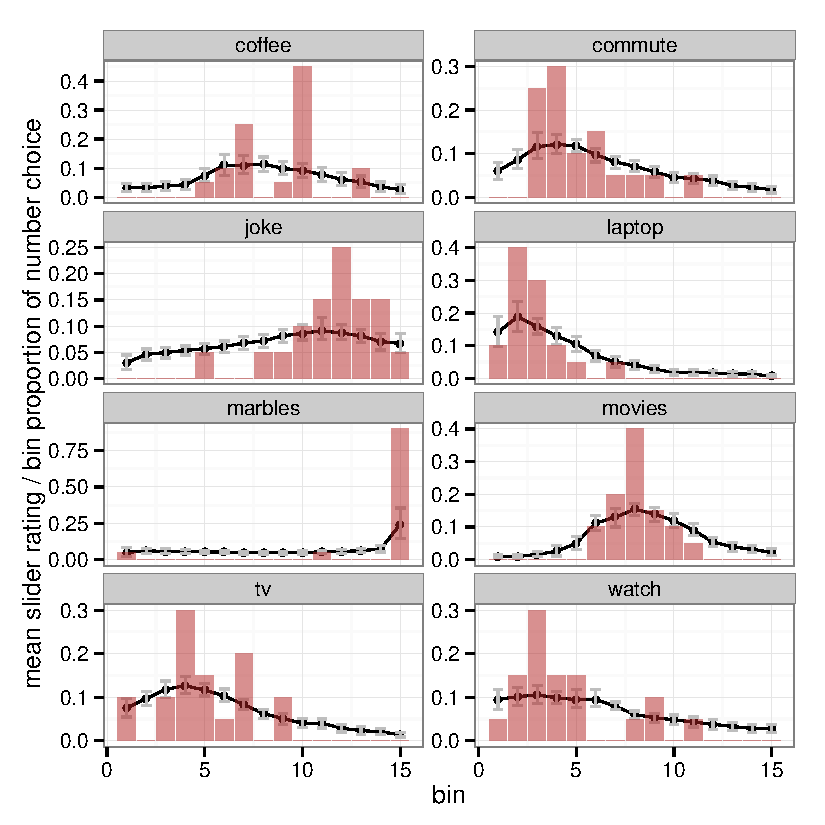
\includegraphics[width = \textwidth]{plots/data_sliderNumber.pdf}
    \caption{Red: proportion of choosing a number in each bin on \emph{give-a-number} trials. Black: mean slider ratings on \emph{binned histogram} trials.}
    \label{fig:slider}
  \end{subfigure}

  \begin{subfigure}[b]{0.5\textwidth}
    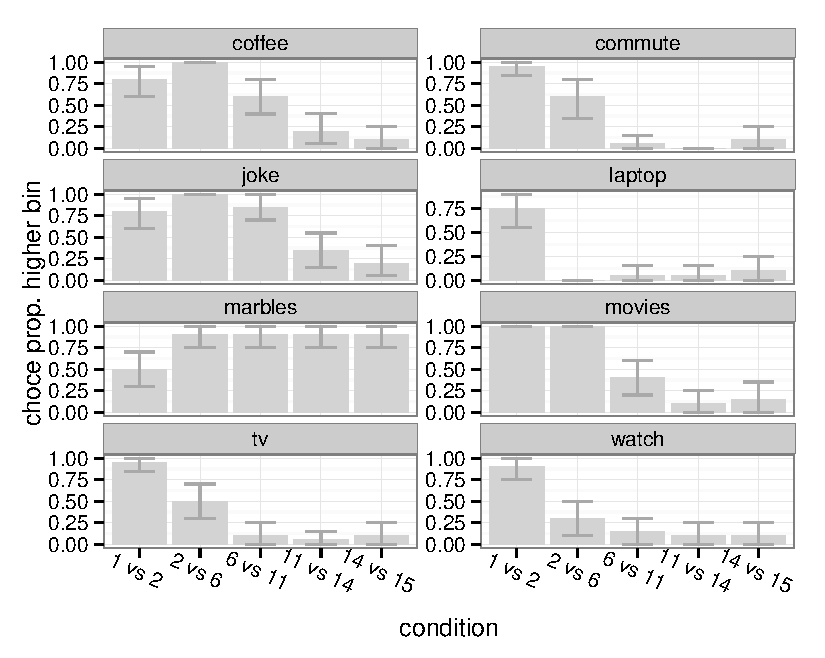
\includegraphics[width = \textwidth]{plots/data_choice.pdf}
    \caption{Proportion of choosing the higher bin on \emph{paired comparison} trials.}
    \label{fig:lighting}
  \end{subfigure}

  \caption{Experimental results. Error bars show bootstrapped 95\% confidence intervals.}
  \label{fig:Results}
\end{figure}


\section{Model}

The data we would like to explain are: (i) the normalized slider ratings $s_{ijk} \in [0;1]$ of
participant $i \in \set{1, \dots, 20}$ for item $j \in \set{1, \dots, 8}$ and bin
$k \in \set{1, \dots, 15}$ from the binned histogram task; (ii) the bins $n_{ij} \in \set{1, \dots, 15}$ in which participant
$i$'s number choice for item $i$ was in the give-a-number task; and (iii) the binary choices $c_{ijl} \in \set{0,1}$ of
whether participant $i$ selected the higher bin for item $j$ in the paired comparison task for each comparison
$l$. There are two simplifications in need of commenting. In (i), we focus on slider ratings after
normalizing for each participant, because we assume that slider adjustments reflect relative, not
absolute estimates of subjective beliefs. In (ii), we focus on bin choices, not actual number
choices, in order to avoid, as much as possible, considerations of salience of particular
numbers, and also because otherwise data from items with smaller domains of plausible numbers
would get more weight than data from items which allow for a wider set of number choices.

All three pieces of data are to be explained as functions of subjective beliefs $P_{ij}$, where
$P_{ij}$ is a probability vector of length 15 with $P_{ijk}$ being participant $i$'s belief about
the relative likelihood of bin $k$ for item $j$. Each $P_{ij}$ defines a likelihood for our
data, via appropriate link functions (to be spelled out presently). Variance in subjective
beliefs is harnessed by a population-level hyper-prior with central tendency $Q_{j}$, i.e., a
stochastic vector of length 15, which we call a ``population-level belief'' about item $j$. The
structure of this model is pictured in \figref{fig:ModelGraph}.

\begin{figure}[]
  \centering
  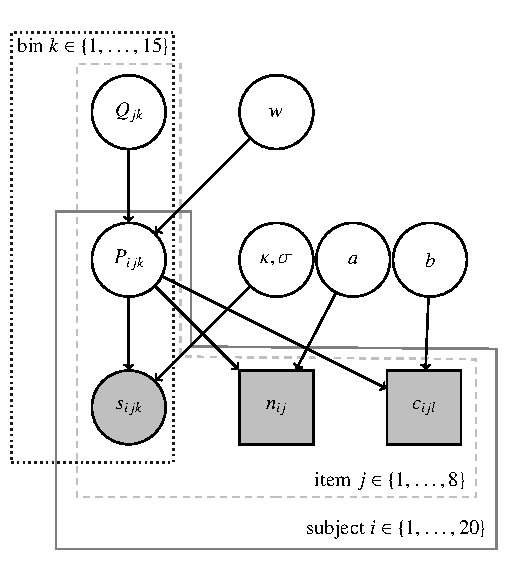
\includegraphics[width = 0.4\textwidth]{modelGraph/modelGraphNoMath.pdf}
  \caption{The data-generating model as a probabilistic graphical model, following conventions
    of \citet{LeeWagenmakers2013:Bayesian-Cognit}. Shaded nodes are observed, white nodes are
    latent variables. Square nodes represent categorical, round nodes continuous
    variables. Boxes indicate scope of indices.}
  \label{fig:ModelGraph}
\end{figure}

To fill the structure in Figure~\ref{fig:ModelGraph} with life, we need to spell out three
parameterized link functions, one for each task type, and the relation between population-level
belief $Q_j$ to individual beliefs $P_{ij}$. Let's start with the latter. For fixed $Q_j$, the
idea is that $P_{ij}$ are noise-perturbed variants scattered around $Q_j$, with some parameter
$w$ to determine how much perturbation we should expect. To realize this, the model assumes
that $P_{ij}$ are distributed according to a Dirichlet distribution with weights given by
$w Q_{j}$:
\begin{align*}
  Q_j & \sim \text{Dirichlet}(1, \dots, 1) & w & \sim \text{Gamma}(2,0.1) \\
  P_{ij} & \sim \text{Dirichlet}( w Q_j)
\end{align*}
The higher $w$, the more likely it is that $P_{ij}$ is ``close'' to $Q_j$.

The link function for the slider rating data uses a logit transformation to project observed
slider ratings $s_{ijk}$ and latent probabilities $P_{ijk}$, which are bound to lie between 0
and 1, to the reals. The likelihood of logit-transformed observation $s_{ijk}$ is given by a
Gaussian with standard deviation $\sigma$ around the logit-transformed predictor $P_{ijk}$. On
top of that, there is a parameter $\kappa$, the steepness of the logit transform of $P_{ijk}$,
that allows response likelihoods to capture end-point affinity for $\kappa >1$ (values of
$P_{ijk}$ close to 0 or 1 are likely mapped to 0 or 1) or end-point aversion for $\kappa <0$
(values of $P_{ijk}$ are likely to be realized as more median), with a prior that expects
$\kappa=1$.
\begin{align*}
  \text{logit}(s_{ijk}) &\sim
        \text{Norm}(\text{logit}(P_{ijk}, \kappa), \sigma) \\
        \sigma &  \sim \text{Gamma}(0.0001,0.0001) & \kappa &\sim \text{Gamma}(5,5)
\end{align*}
 
The link function for number choice data treats each bin $n_{ij}$ as a draw from a categorical
distribution where the probability of bin $k$ is proportional to $\expo(a P_{ij})$, i.e., a
soft-max choice from $P_{ij}$. The higher parameter $a$, the more likely $n_{ij}$ is the mode
of $P_{ij}$. For $a \rightarrow 0$, all bins become equiprobable.
\begin{align*}
  n_{ij} & \sim
        \text{Categorical}(\expo(a P_{ij})) &
 a & \sim \text{Gamma}(2,1)
\end{align*}

Finally, consider the link function for bin comparisons. We are interested in the likelihood with which
participant $i$ selects the higher bin for item $j$ in bin comparison condition $l$. Suppose $l$ is
about comparing the lower bin $b_l$ to the higher $b_h$. The perhaps most natural approach
would be to link the likelihood of choosing $b_h$ over $b_l$ to the difference between
$P_{ijb_h}$ and $P_{ijb_l}$. This, however, does not appear to be what participants were doing. For
example, take the ``marbles'' case where we see almost unanimous choices of bin 11 over bin 6,
despite seeing no pronounced difference in slider ratings for these bins. Indeed, a model that
implements this idea failed to capture the relevant regularities in the data blatantly.

Another plausible link function that accommodates for this is to assume that what matters in
bin comparisons is the distance to the mode of $P_{ij}$: soft-max prefer the bin that is closer
to the mode of $P_{ij}$; select randomly if both bins are equally far from the
prototype.\footnote{Notice that
  $(1 + \exp(2b(1-p^{\text{high}}_{ijl})) )^{-1} = \frac{\exp(b p^{\text{high}})}{\exp(b
    p^{\text{high}}) + \exp(b p^{\text{low}})}$
  with $p^\text{low}_{ijl} = 2 - p^\text{high}_{ijl}$.}
\begin{align*}
  c_{ijl} & \sim \text{Bern}( (1 + \exp(2b(1-p^{\text{high}}_{ijl})) )^{-1} ) \ \ \ 
  b  \sim \text{Gamma}(2,1) \\
  p^\text{high}_{ijl} & = \begin{cases}
    2 & \text{if $mode(P_{ij})$ is closer to higher} \\
    & \text{ bin of $l$ than to lower bin } \\ 1 & \text{if equal
      distance} \\ 0 & \text{otherwise}  
  \end{cases}
\end{align*}

\ndg{wow, this is weird! you tried softmax ratio of bin probs?}

\jd{hm, doesn't seem too weird to me!}

\section{Inference}

The model was implemented in JAGS \cite{Plummer2003:JAGS:-A-Program}. 50,000 samples were
obtained from two chains with a thinning rate of 2 after a burn-in of 100,000 that ensured
convergence according to $\hat{R}$ \cite{GelmanRubin1992:Inference-from-}.

Of most theoretical interest are posterior estimates of $Q_j$. Figure~\ref{fig:PosteriorQj}
shows means of the posterior $Q_j$, with their 95\% HDIs, alongside the averaged normalized
slider ratings. The latter provide a very good approximation of the latent, inferred
population-level beliefs. Inspection of posteriors of individual $P_{ij}$ shows that there is
ample variation between participants. Nonetheless, the way the model suggest we should think about
harnessing the individual $P_{ij}$s under a population-level central tendency is closely
approximated by simply averaging over slider ratings. Although the match is clearly not
perfect, it is good enough to maintain that the latter are a reasonable (enough) and practical
way of assessing what the crowd believes despite individual differences.

\ndg{it'd be nice to see some posteriors for some of the (more meaningful) parameters. eg w, kappa, ...}

\ndg{what about the success of the other DMs? looks like give-n is not so hot. worth saying that if so.}

\begin{figure}
  \centering
  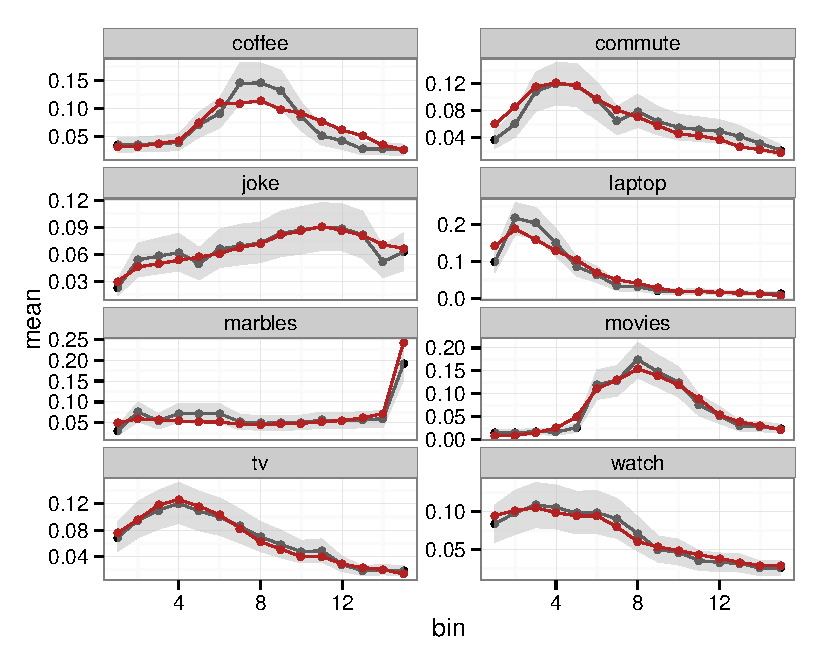
\includegraphics[width = 0.5\textwidth]{plots/pop_priors.pdf}
  \caption{Means of posteriors over $Q_j$ in black with gray area indicating 95\% HDIs. Red
    lines give the average normalized slider ratings for comparison.}
  \label{fig:PosteriorQj}
\end{figure}

\section{Model criticism}

Inferences based on the model are only as reliable as the model itself is plausible. Model
criticism is therefore important. Figure~\ref{fig:PPCs} shows posterior predictive checks at
the population-aggregate level for all of our three task types. For the binned histogram task,
posterior predictions are spot-on. Some of the give-a-number data is surprising even for
the model trained on this very data. This could have various reasons: (i) the give-a-number data does
not have a huge influence on the posterior likelihood, (ii) number choices may be influenced by
saliency and/or roundness of numbers after all. Finally, there is one condition in the paired
comparison task that the model definitely got wrong. This is the choice of what is more likely:
that one or that none of 14 marbles thrown into a pool would sink. The model would predict that
almost everybody should answer that it is more likely that one marble sank. But that is not
what we observe. It may be that participants revise beliefs about ``normality'' of the marbles,
while holding on to an assumption that all marbles behave in the same way 
\cite{DegenTessler2015:Wonky-worlds:-L}.

\begin{figure}
  \centering
  \begin{subfigure}[b]{0.5\textwidth}
    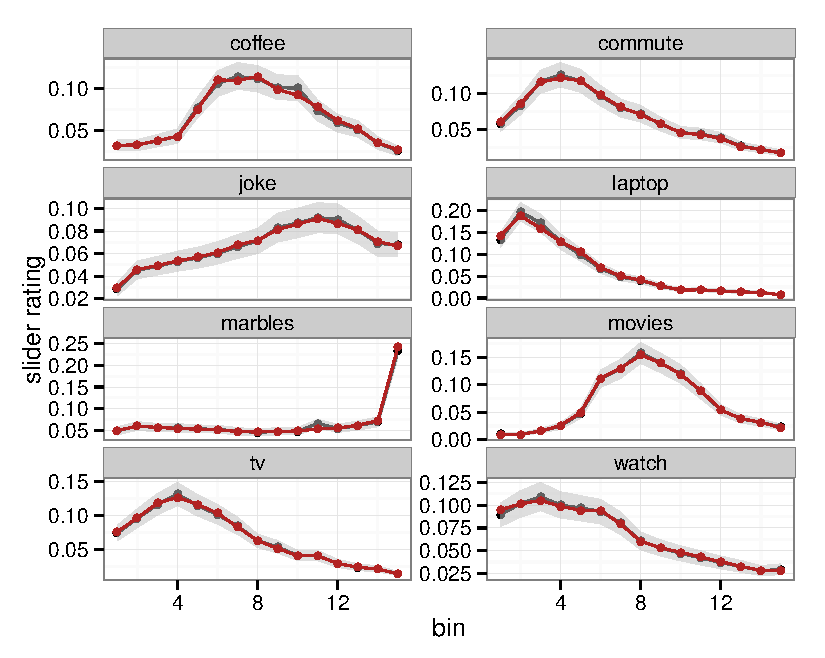
\includegraphics[width = \textwidth]{plots/ppc_slider.pdf}
    \caption{Binned histogram task.}
    \label{fig:sliderPPC}
  \end{subfigure}
   
  \begin{subfigure}[b]{0.5\textwidth}
    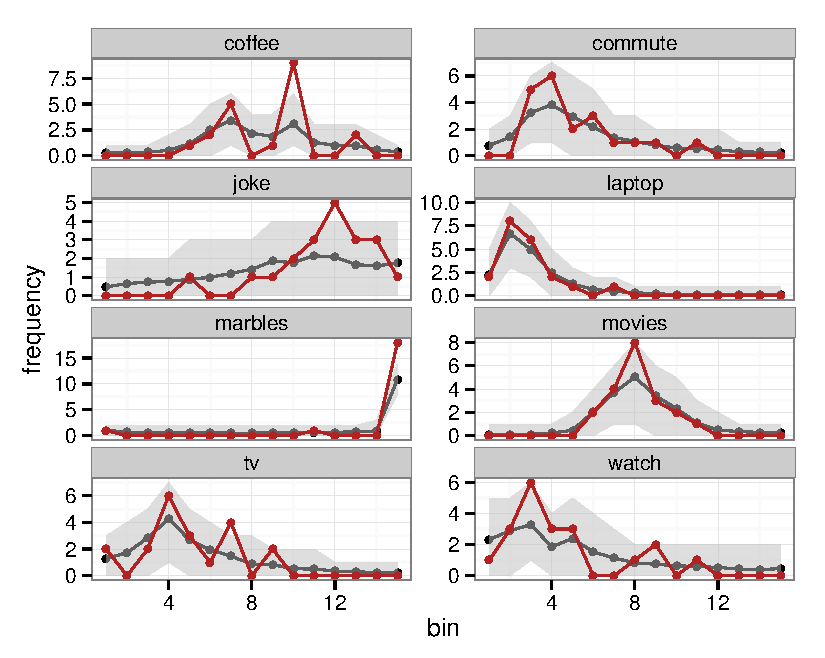
\includegraphics[width = \textwidth]{plots/ppc_number.pdf}
    \caption{Give-a-number task.}
    \label{fig:numberPPC}
  \end{subfigure}

  \begin{subfigure}[b]{0.5\textwidth}
    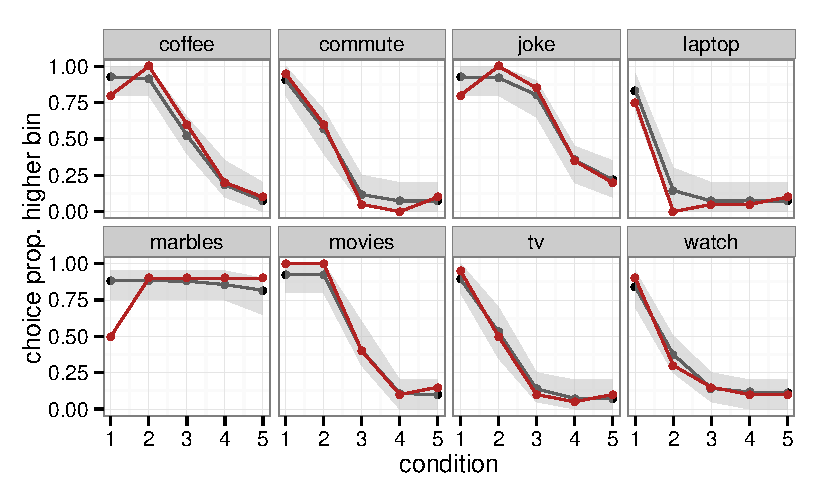
\includegraphics[width = \textwidth]{plots/ppc_choice.pdf}
    \caption{Paired comparison task.}
    \label{fig:lightingPPC}
  \end{subfigure}

  \caption{Posterior predictive checks for aggregate data. Red lines give empirical
    observations. Black lines are means of posterior predictive samples, gray areas are
    95\% HDIs.}
  \label{fig:PPCs}
\end{figure}

Posterior predictive checks indicate that the trained model captures patterns of answers at the
aggregate population level well. To have a more fine-grained measure of model fit, we also
looked at posterior predictive $p$-values at the level of participants and items. \ndg{need to say what this means -- i'm not even sure that i know!} Unfortunately,
only the slider rating task provides enough data for such a fine-grained analysis. For the
slider rating task, fixing a participant and an item, observations and replicates are probability
vectors of length 15. In a first analysis, we used the mean of these probability vectors as a
test statistic. The minimum posterior predictive $p$-value over all 20 (participants) times 8
(items) cases was 0.13, suggesting that the means of observed $s_{ij}$ are non-surprising to
the trained model. In a second analysis, we used entropy as a test statistic. Two cases gave
posterior predictive $p$-values lower than 0.05. These were from the two participants who gave a
very extreme slider rating for the ``marbles'' item, basically assigning all ``mass'' to the
last bin. What this suggests is that the model can cope reasonably well also with
individual-level data, but has problems accounting for ``extreme'' choices, given that the
population-level hyper-prior on $P_{ij}$ will lead to shrinkage.
\ndg{can say that one possibility (future work) would be to switch to a fatter-tailed distribution relating Q to P, in order to deal with outliers.}

\section{Conclusions}

\begin{itemize}
\item \ndg{say more clearly that we focus on unidimensional distributions and why.}
\end{itemize}


\section{Acknowledgments}

MF's work was supported by the Institutional Strategy of the University of T̈\"{u}bingen (Deutsche
Forschungsgemeinschaft, ZUK 63). MF and JD's work was supported by the Priority Program XPrag.de (DFG Schwerpunktprogramm
1727). This work was further supported by ONR grant N00014-13-1-0788 and a James S. McDonnell Foundation Scholar Award to NDG and an SNF Early Postdoc.Mobility Award to JD.



\bibliographystyle{apacite}

\setlength{\bibleftmargin}{.125in}
\setlength{\bibindent}{-\bibleftmargin}

\bibliography{references}


\end{document}
